\documentclass[12pt,a4paper]{article}
\usepackage{mathptmx} % added for time new roman font
\usepackage[left=0.5in,right=0.5in,top=1in,bottom=1in]{geometry}
\usepackage[latin1]{inputenc}
\usepackage{amsmath}
\usepackage{amsfonts}
\usepackage{amssymb}
\usepackage{graphicx}
\usepackage{float}
\usepackage{booktabs}
\usepackage{parskip} % remove all the paragraph indents


\usepackage{setspace}
\usepackage[colorlinks=true]{hyperref}
\usepackage{textcomp} 
\usepackage{multicol} 

\usepackage{mathtools}          %loads amsmath as well added for the piece wise function
\DeclarePairedDelimiter\Floor\lfloor\rfloor
\DeclarePairedDelimiter\Ceil\lceil\rceil

 
\newcounter{NumberInTable}
\newcommand{\LTNUM}{\stepcounter{NumberInTable}{(\theNumberInTable)}}

\newcommand{\Laplace}[1]{\ensuremath{\mathcal{L}{\left[#1\right]}}}
\newcommand{\InvLap}[1]{\ensuremath{\mathcal{L}^{-1}{\left[#1\right]}}}
\renewcommand{\textuparrow}{$\uparrow$}

\begin{document}
	
	\large{}
	
	\title{\vspace{-2cm}Lecture Notes, Topic-3}
	\date{}
	\maketitle
	
	\section*{Review from previous class}
		\begin{enumerate}
			\item Solved the ODE (EOM) through observing a vibrating system
			\item Obtain an equation for the free response of a system
		\end{enumerate}
	
	\section*{Objectives for today's class}
		\begin{enumerate}
			\item Review Euler's (pronounced oy-ler) formula
			\item Obtain a general solution for vibrating systems
		\end{enumerate}
		
	\section*{Lecture}

		\subsection*{Review of complex numbers.}
			Vibration analysis uses complex numbers to solve the EOM's differential equation. In this class the imaginary number is termed $j$ (sometimes referred to as $i$): such that:
			
			\begin{equation}
				j = \sqrt{-1}
			\end{equation}		
			and:	 
			\begin{equation}
				j^2 = -1
			\end{equation}	
			a general complex number. $x$ can be expressed as 
			\begin{equation}
				x=a+bj
			\end{equation}			 	
			here, $a$ is referred to as the real number and $b$ is the imaginary part of the number $x$. Such complex numbers can be represented in the complex plane, also called a Argand plot. The absolute value or modules is defined as $|x|$ presented on the Argand plot. 
			
			\begin{figure}[H]
				\centering
				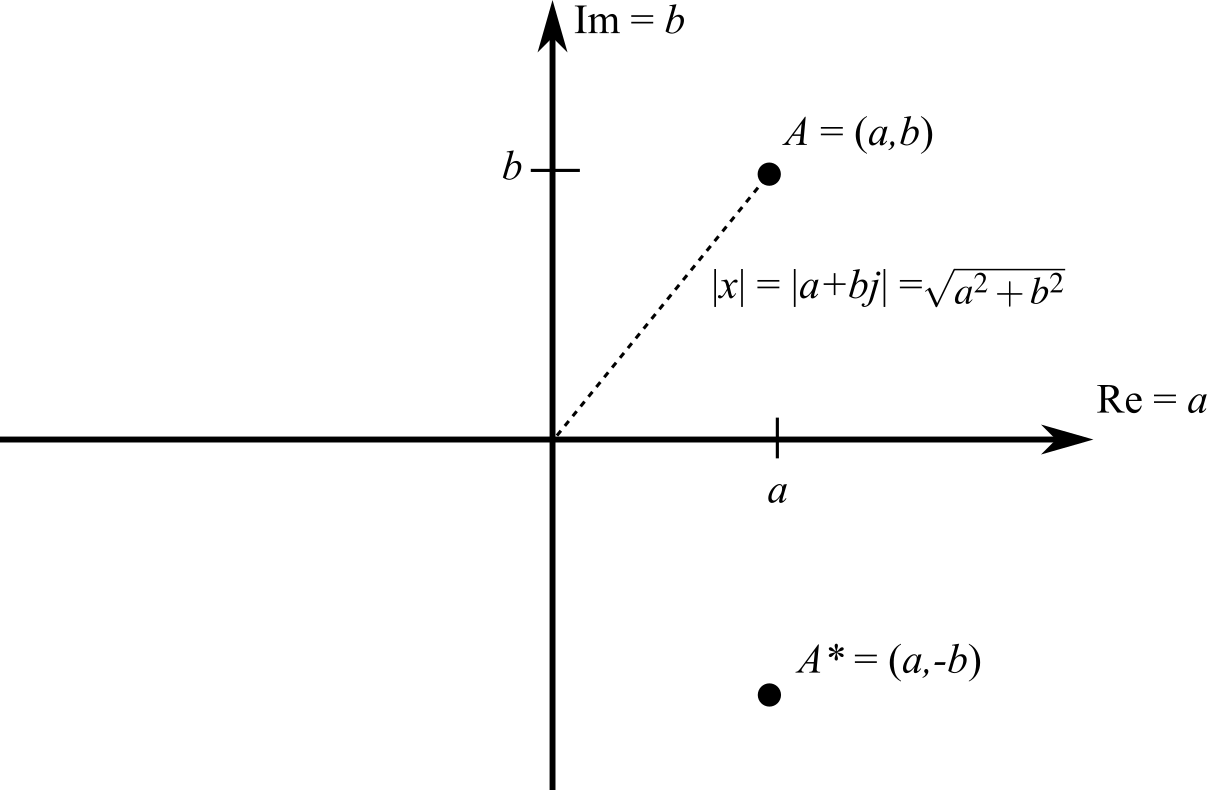
\includegraphics[width=0.5\textwidth]{../../Figures/complex_plane.png}
			\end{figure}
					
			$A$ and $A^*$ prime are complex conjugate pairs. In mathematics, the complex conjugate of a complex number is the number with an equal real part and an imaginary part equal in magnitude but opposite in sign. In other words, a conjugate pair is $a + bj$ and $a - bj$.  
			
			Definition $\rightarrow$ \textbf{con�ju�gate} (adjective): Coupled, connected, or related.
			
		\subsection*{Review of Euler's formula.}
		
			Euler's formula, named after Swiss engineer and mathematician Leonhard Euler (1707-1783), is a mathematical formula in complex analysis that establishes the fundamental relationship between the trigonometric functions and the complex exponential function. Euler's formula states that for any real number $x$,
			\begin{equation}
				e^{j\psi} = \text{cos}(\psi) + j \text{sin}(\psi)
			\end{equation}		
			where $j=\sqrt{-1}$. This equation can also be expressed as:
			\begin{equation}
				e^{-j\psi} = \text{cos}(\psi) - j \text{sin}(\psi)
			\end{equation}	
			This can be expressed in terms of polar coordinates as:				
			\begin{figure}[H]
				\centering
				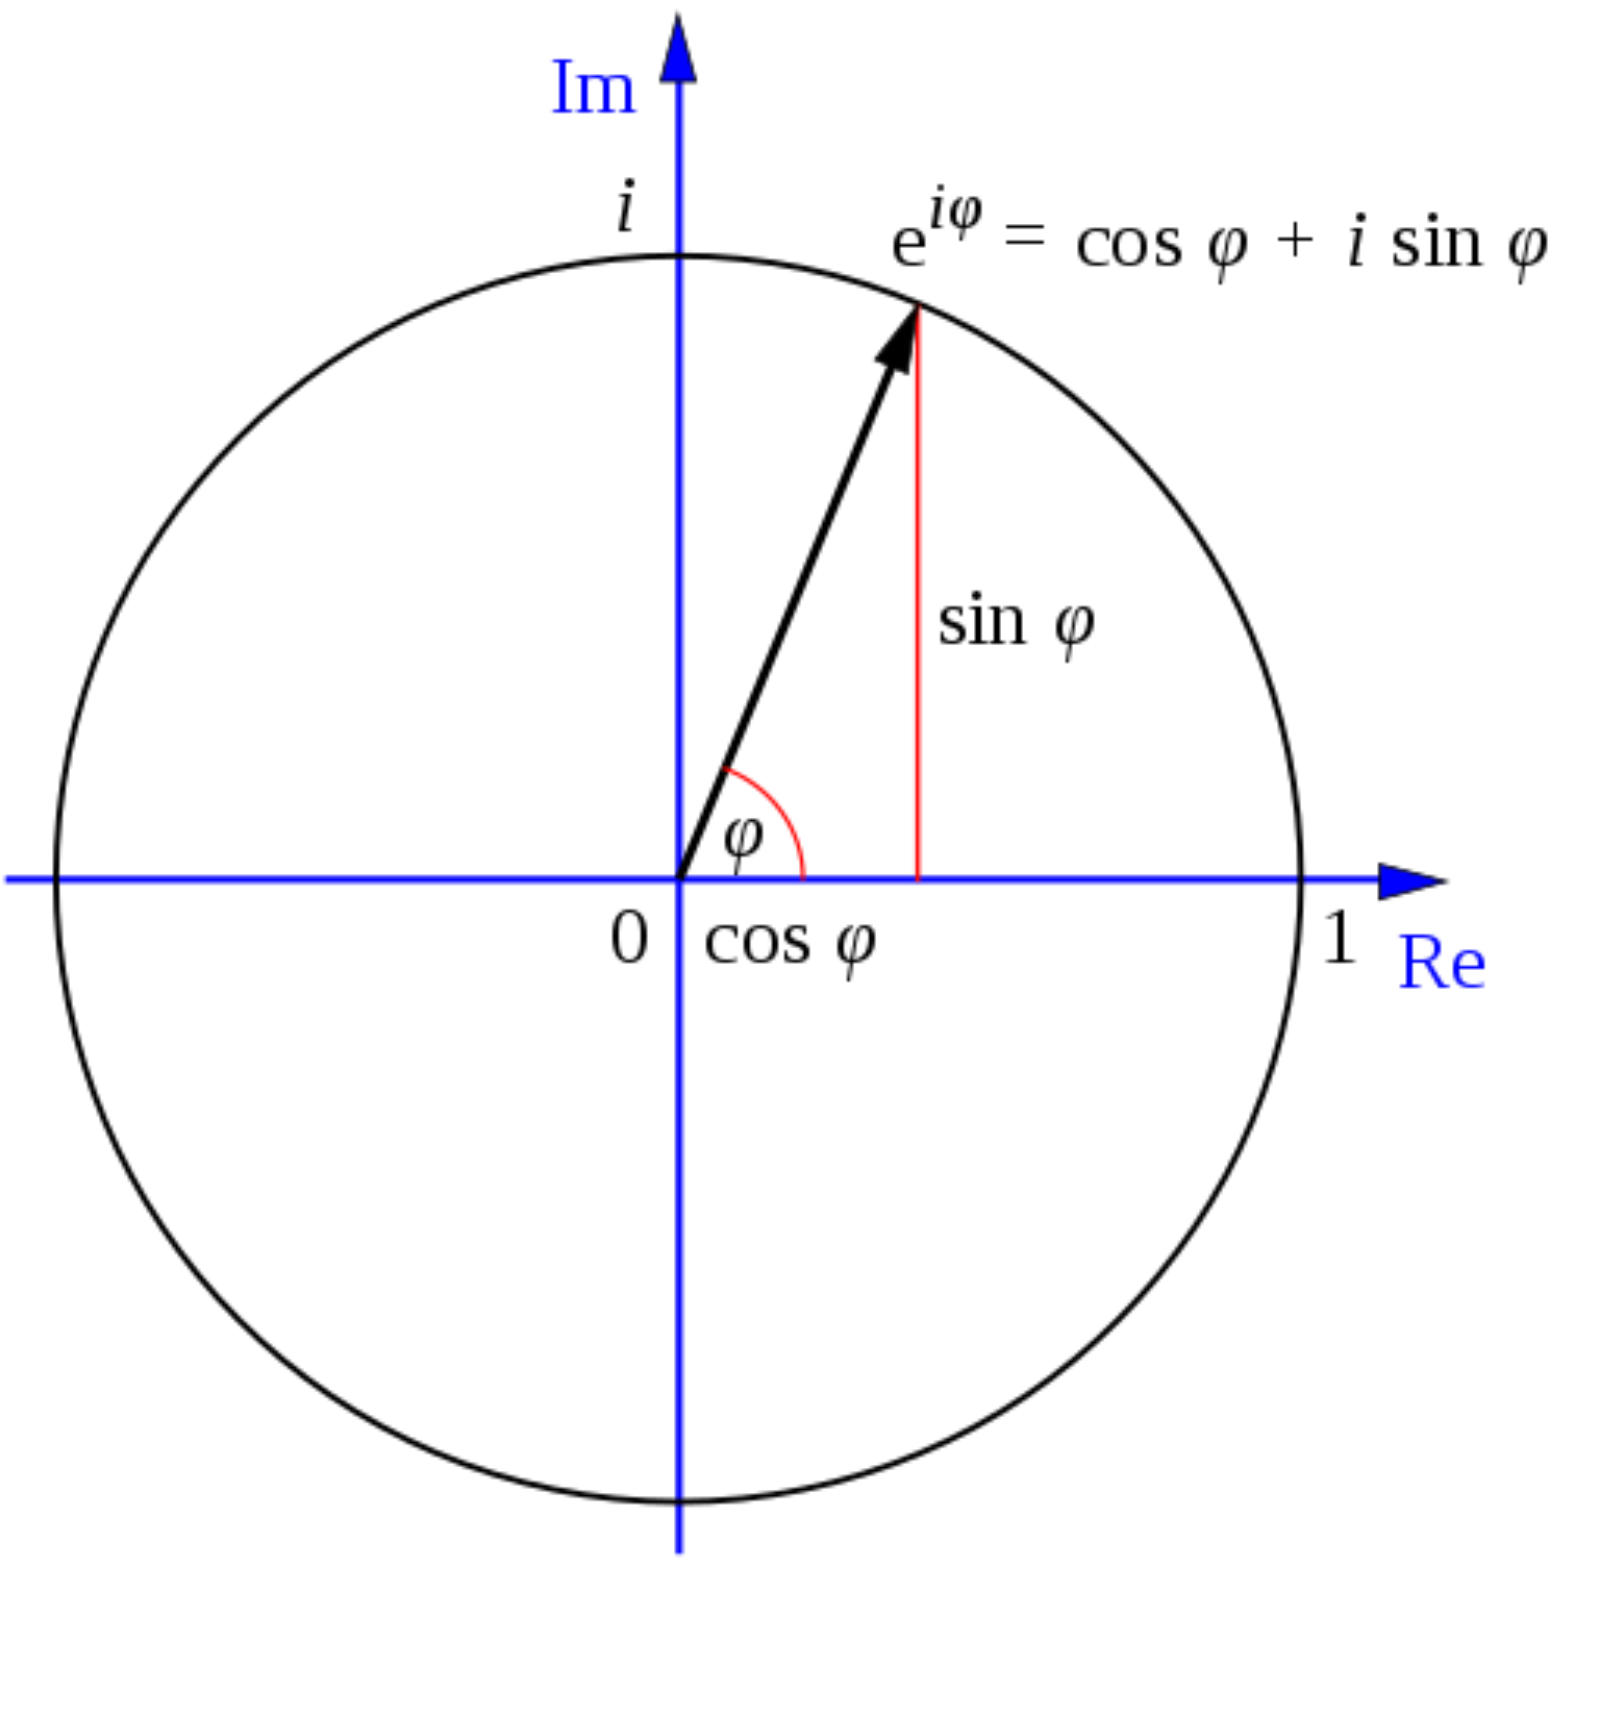
\includegraphics[width=0.4\textwidth]{../../Figures/Euler's_formula.png}
			\end{figure}
	
		\subsection*{Theory of elementary differential equations. }
			We can also solve the following EOM:
			\begin{equation}
				m\ddot{x}+kx=0
			\end{equation}		
			in a more analytical manner using the theory of elementary differential equations. To do this we have to assume a solution, in the form of 
			\begin{equation}
				x(t) = ae^{\lambda t}
			\end{equation}
			here, $a$ and $t$ are nonzeros constants that need to be determined.  Using successive differentiation, we get:
			\begin{equation}
				\dot{x}(t) = \lambda ae^{\lambda t}
			\end{equation}
			and 
			\begin{equation}
				\ddot{x}(t) = \lambda^2 ae^{\lambda t}
			\end{equation}
			therefore, $m\ddot{x}(t) + kx(t) = 0$ becomes:
			\begin{equation}
				m \lambda^2 ae^{\lambda t}  + k ae^{\lambda t} = 0
			\end{equation}
			Now we divide by $ae^{\lambda t}$ to obtain the \textbf{characteristic equation}:
			\begin{equation}
				m \lambda^2 + k = 0
			\end{equation}
			We can do this because $ae^{\lambda t}$ is never zero, therefore, we never divide by zero. The quadratic formula gives us:
			\begin{equation}
				\lambda = \pm \sqrt{-\frac{k}{m}} = \pm \sqrt{\frac{k}{m}}j = \pm \omega_n j
			\end{equation} 
			remember that $\omega_n = \sqrt{\frac{k}{m}}$. Notice that the $\pm$ tells us there are two solutions to this problem. So, putting $\lambda$ back into our assumed solution, we get two solutions:   
			\begin{equation}
				x(t) = a_1e^{+\omega_n j t}
			\end{equation}
			and 
			\begin{equation}
				x(t) = a_2e^{-\omega_n j t}
			\end{equation}
			As we deal with linear systems, we know that the sum of the solutions is also a solution, resulting in:
			\begin{equation}
				x(t) = a_1e^{+\omega_n j t} + a_2e^{-\omega_n j t}
			\end{equation}
			where $a_1$ and $a_2$ are complex valued constants of integration. This equation derived using Euler's formula is equivalent to the $A\text{sin}(\omega_n+\phi)$. To recover the previously assumed solution we apply the knowledge that $a_1$ and $a_2$ are complex congregate pairs and as such the magnitude can be expressed as $a_1=a_2$. Using Euler's polar notation, $a_1$ and $a_2$ can be expressed as 
			\begin{equation}
				a_1 = a_2 = ae^{j\psi}
			\end{equation}	
			where $a$ and $\psi$ are real numbers, the equation becomes:		
			\begin{equation}
				x(t) = ae^{j(\omega_n t+\psi)} + ae^{-j(\omega_n t+\psi)}
			\end{equation}			
			this becomes:
			\begin{equation}
				x(t) = a(e^{j(\omega_n t+\psi)} + e^{-j(\omega_n t+\psi)})
			\end{equation}				
			Remembering Euler's equations from before, this becomes:
			\begin{equation}
				x(t) = a\big(\text{cos}(\omega_n t+\psi) + j \text{sin}(\omega_n t+\psi) + \text{cos}(\omega_n t+\psi) - j \text{sin}(\omega_n t+\psi)\big)
			\end{equation}				
			combining the ``cos'' terms and canceling out the ``sin'' terms this becomes:
			\begin{equation}
				x(t) = 2a \cdot \text{cos}(\omega_n t+\psi)
			\end{equation}						
			This is equivalent to $	{x}(t) = A\text{sin}(\omega_n t + \phi)$ if we take $A=2a$ and knowing sin($\phi$) = cos($\phi + \psi$).
			
		\subsection*{Formulate the general solution from Euler's expression. }						
			From Euler's equation we saw that:
			\begin{equation}
				x(t) = a_1e^{+\omega_n j t} + a_2e^{-\omega_n j t}
			\end{equation}			
			we can expand this into the form: 
			\begin{equation}
				x(t) = a_1\big(\text{cos}(\omega_n t) + j \text{sin}(\omega_n t)\big) + a_2\big(\text{cos}(\omega_n t) - j \text{sin}(\omega_n t)\big)
			\end{equation}
			using trigonometric functions. This equates to:
			\begin{equation}
				x(t) = (a_1+a_2) \cdot \text{cos}(\omega_n t) + (a_1-a_2)j \cdot \text{sin}(\omega_n t)
			\end{equation}			
			as $x(t)$ is always real, we can define:
			\begin{equation}
				A_1 = (a_1+a_2)
			\end{equation}		
			and
			\begin{equation}
				A_2 = (a_1-a_2)j
			\end{equation}	
			lastly, as the \textbf{general solution} is written as:
			\begin{equation}
				x(t) = A_1\text{cos}(\omega_n t) + A_2\text{sin}(\omega_n t)
			\end{equation}	
			This is the general solution for the EOM ($m\ddot{x}+kx=0$) of the considered oscillating system where $A_1$ and $A_2$ are defined as:
			\begin{equation}
				A = \sqrt{A_1^2+ A_2^2}
			\end{equation}
			and	
			\begin{equation}
				\phi = \text{tan}^-1\bigg(\frac{A_1}{A_2}\bigg)
			\end{equation}		
			These are obtained from a trigonometric relationship, similar to that used before:
			\begin{figure}[H]
				\centering
				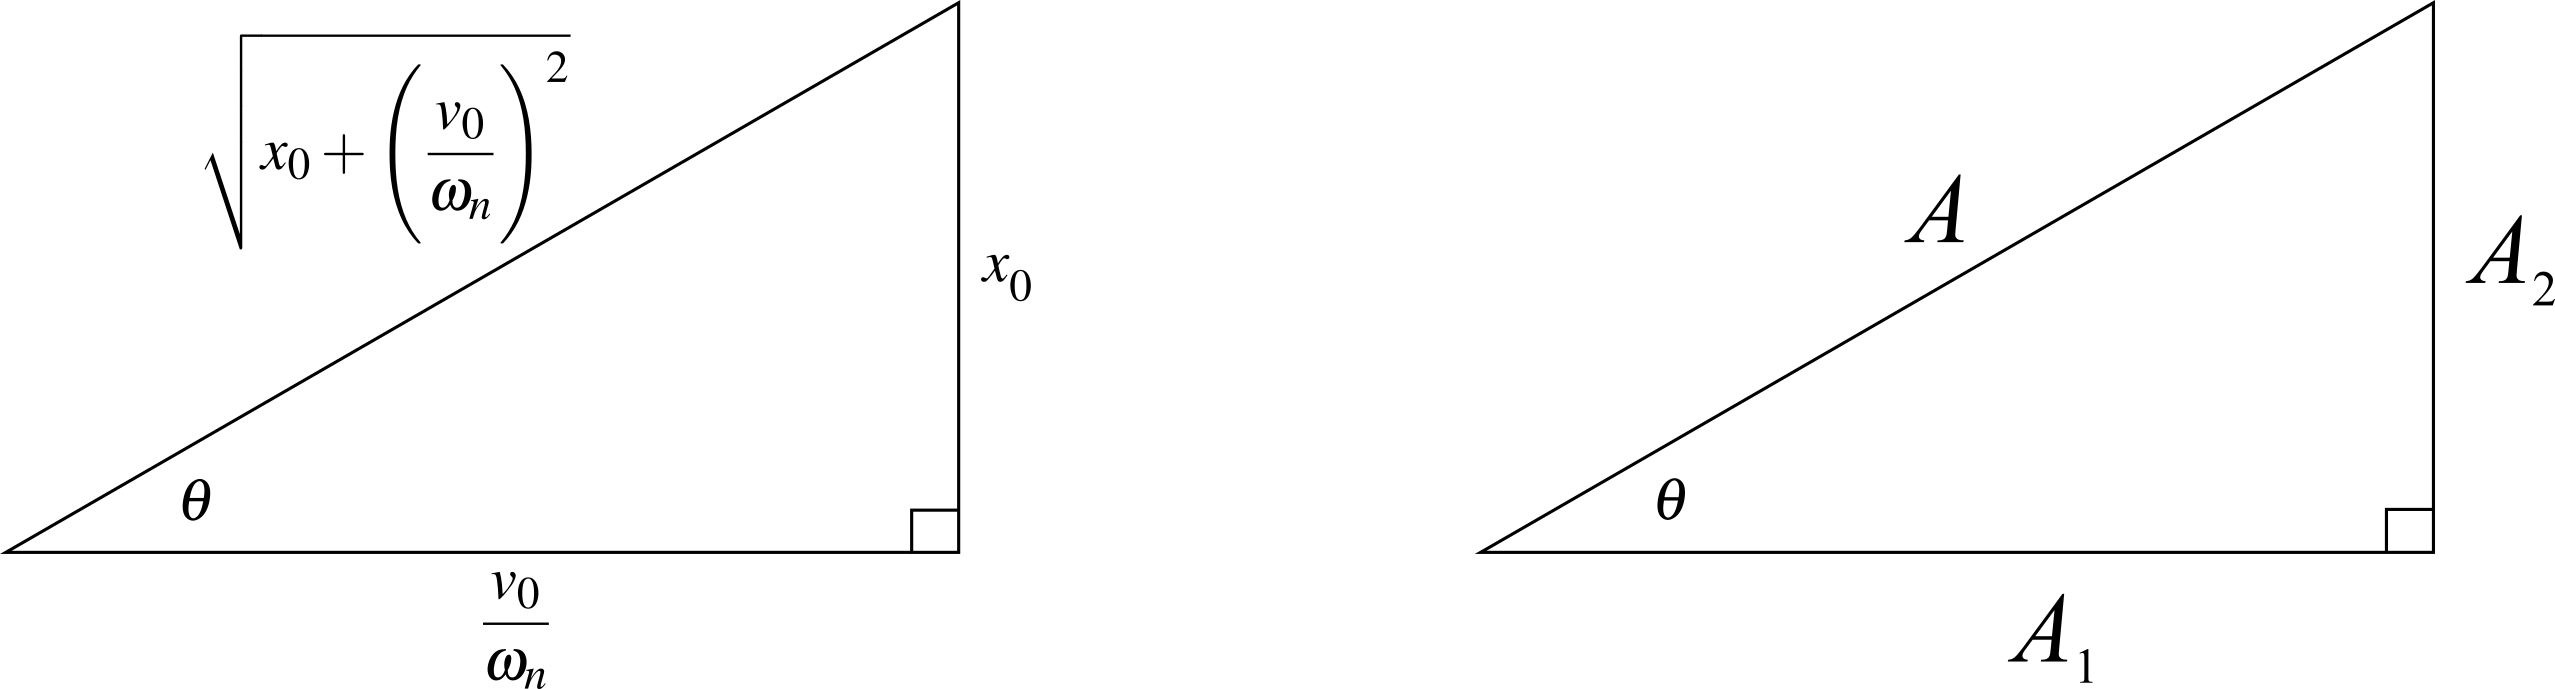
\includegraphics[width=0.8\textwidth]{../../Figures/Trigonometric_relationship_A_theta_A1_A.png}
			\end{figure}
			again, $A$ and $\phi$ are:
			\begin{equation}
				A = \frac{\sqrt{\omega_n^2x_0^2+v_0^2}}{\omega_n} = \sqrt{x_0^2+\Bigg(\frac{v_0}{\omega_n}\Bigg)^2}
			\end{equation}
			\begin{equation}
				\phi = \text{tan}^{-1}\bigg(\frac{x_0\omega_n}{v_0}\bigg)
			\end{equation}		

		\subsection*{One Equation in three forms:}
			Form one, for $m\ddot{x} + kx =0$ subject to nonzero initial conditions can be written as:  		
			\begin{equation}
				x(t) = a_1e^{+\omega_n j t} + a_2e^{-\omega_n j t}
			\end{equation}	
			where $a_1$ and $a_2$ are complex terms. Form two is:
			\begin{equation}
				{x}(t) = A\text{sin}(\omega_n t + \phi)
			\end{equation}
			while form three is:
			\begin{equation}
				x(t) = A_1\text{cos}(\omega_n t) + A_2\text{sin}(\omega_n t)
			\end{equation}	
			where $A$, $\phi$, $A_1$, and $A_2$, are all real-valued constants. Each set of constants can be related to each other by:
			\begin{align}
				A = \sqrt{A_1^2+ A_2^2} & \hspace{1.5cm} \phi = \text{tan}^-1\bigg(\frac{A_1}{A_2}\bigg) \\
				A_1 = (a_1+a_2) & \hspace{1.5cm} A_2 = (a_1-a_2)j \\
				a_1 = \frac{A_1-A_2j}{2} & \hspace{1.5cm} a_2 = \frac{A_1+A_2j}{2}
			\end{align}
			Which follow from trigonometric identities and the Euler's formulas. 
		
		\subsection*{Example 1}	Using the general solution: 
			\begin{equation}
				x(t) = A_1\text{cos}(\omega_n t) + A_2\text{sin}(\omega_n t)
			\end{equation}			
			Calculate the values of $A_1$ and $A_2$ in terms of their initial conditions $x_0$ and $v_0$.
			
			\noindent\textbf{Solution:} Knowing the following for $x$ and $\dot{x}$:
			\begin{equation}
				x(t) = A_1\text{cos}(\omega_n t) + A_2\text{sin}(\omega_n t)
			\end{equation}	
			\begin{equation}
				\dot{x}(t) = -A_1\omega_n\text{sin}(\omega_n t) + A_2\omega_n\text{cos}(\omega_n t)
			\end{equation}	
			Now apply the initial conditions, $x(0)=0$ and $v(0)=0$, this yields:
			\begin{equation}
				x(0) = x_0 = A_1
			\end{equation}	
			\begin{equation}
				\dot{x}(0)= v_0  =  A_2\omega_n
			\end{equation}
			Solving for $A_1$ and $A_2$ shows us:
			\begin{equation}
				A_1 = x_0 \text{, and } A_2 = \frac{v_0}{\omega_n}
			\end{equation}
			thus:
			\begin{equation}
				x(t) = x_0\text{cos}(\omega_n t) + \frac{v_0}{\omega_n}\text{sin}(\omega_n t)
			\end{equation}				



		\subsection*{Important items from today}
	
			\begin{itemize}
				\item The solution for a vibrating system can be expressed in various forms
				\item These forms relate to each other through Euler's equations
			\end{itemize}






\end{document}